\section{Resultados obtenidos}

En este apartado, observaremos el comportamiento de diferentes técnicas 
empleadas por un agente para encontrar el camino en un laberinto representado 
mediante una matriz. En esta representación, cada celda de la matriz indica
el estado de una posición en el laberinto, donde 0 representa un camino libre,
1 es un muro, "E" denota la entrada y "S" representa la salida. Además,
el agente intenta encontrar una salida siguiendo un orden predefinido: 
arriba, abajo, izquierda, derecha.

\begin{figure}[H]
    \centering
    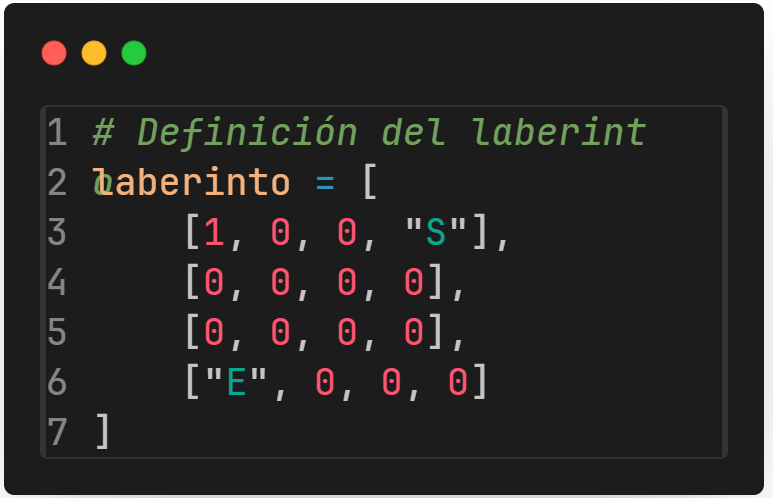
\includegraphics[width=0.4\linewidth]{IMA/laberintoEjemplo.png} 
    \caption{Ejemplar para el agente.} 
\end{figure}

\subsection*{Ejemplos usados}
Como primer ejemplo, se usara un laberinto de 7x7 con la característica de un solo camino en forma
de espiral, en una esquina se encuentra la entrada y en el centro de la matriz se encuentra la salida.
Esto con el fin de dar un ejemplar sencillo para el agente, donde se pueda observar el comportamiento apartir
del algoritmo A*.

\begin{figure}[H]
    \centering
    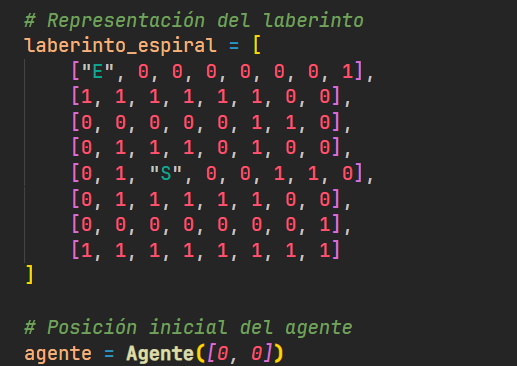
\includegraphics[width=0.5\linewidth]{IMA/Laberinto1.png} 
    \caption{Ejemplar para el agente con un camino en espiral.} 
    \label{fig:ejemplo} 
\end{figure}

En la siguiente imagen se muestra el resultado obtenido por el agente, donde se puede observar que el agente
encuentra el camino más corto para llegar a la salida y las celdas que recorre para llegar a su destino.
Con \textbf{X} se marcan las celdas que recorre el agente para llegar a la salida, con los \textbf{cuadrados} se marcan los muros y con
los \textbf{guion} se marcan las celdas que no recorre el agente.

\begin{figure}[H]
    \centering
    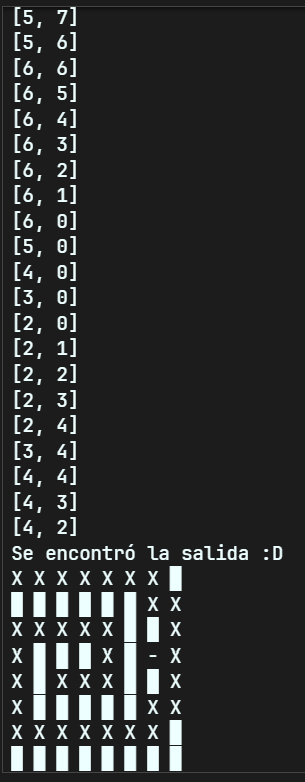
\includegraphics[width=0.2\linewidth]{IMA/RLaberinto1.png} 
    \caption{Ejemplar para el agente con un camino en espiral.} 
    \label{fig:ejemplo} 
\end{figure}

Como segundo ejemplo, se usara un laberinto de 7x7 con la característica que sea simetrico,
es decir, que la entrada y la salida se encuentran en la misma columna y con muros simétricos.

\begin{figure}[H]
    \centering
    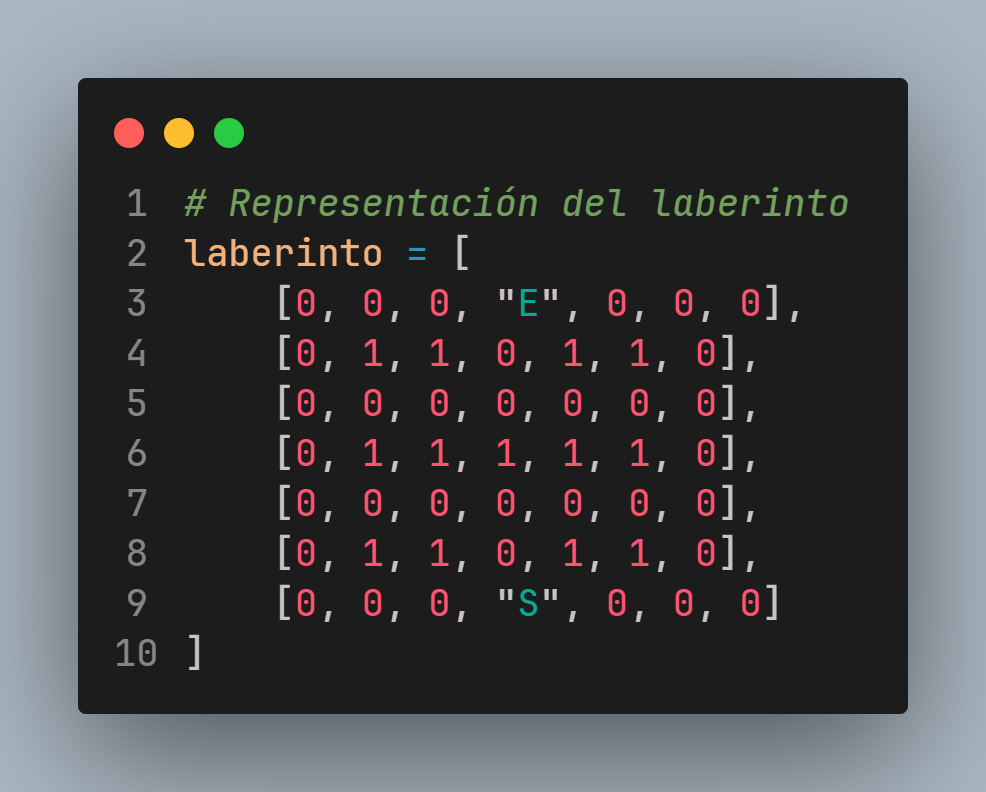
\includegraphics[width=0.4\linewidth]{IMA/Laberinto2.png} 
    \caption{Ejemplar para el agente, con simetría.} 
    \label{fig:ejemplo} 
\end{figure}

Notemos que es posible que el agente encuentre múltiples soluciones viables y evalúe
diferentes caminos hacia la salida. Sin embargo, el algoritmo A* no tiene una lógica
para elegir entre caminos equivalentes cuando varios caminos tienen la misma longitud.
En tales casos, la selección del camino puede depender de la lógica de prioridad implementada 
en el algoritmo.

\begin{figure}[H]
    \centering
    \begin{minipage}[b]{0.2\textwidth}
      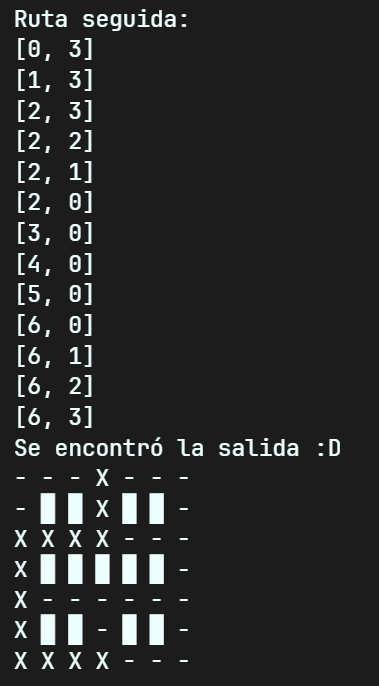
\includegraphics[width=\textwidth]{IMA/RLaberinto2_1.png}
      \caption{Solucion camino por la izquierda}
    \end{minipage}
    \hfill
    \begin{minipage}[b]{0.2\textwidth}
      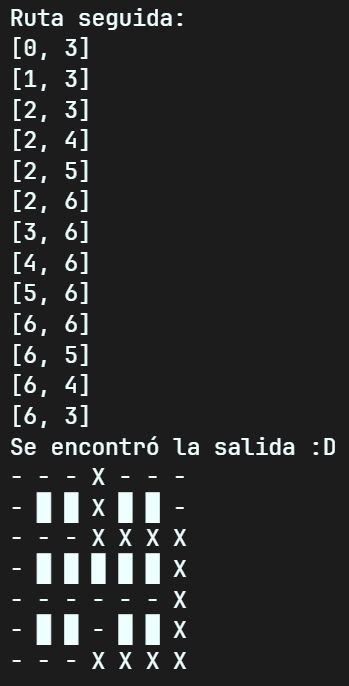
\includegraphics[width=\textwidth]{IMA/RLaberinto2_2.png}
      \caption{Solucion camino por la derecha}
    \end{minipage}
  \end{figure}

El agente encuentra el camino más corto en ambos casos, pero es el orden de la heurística la que establece
la prioridad de los caminos. En esta parte del código, se establece que el agente siempre buscara
primero arriva, abajo, izquierda y derecha, por lo que asiendo el cambio colocando derecha antes que izquierda, el agente
encontrara el camino más corto por la derecha.

\begin{figure}[H]
    \centering
    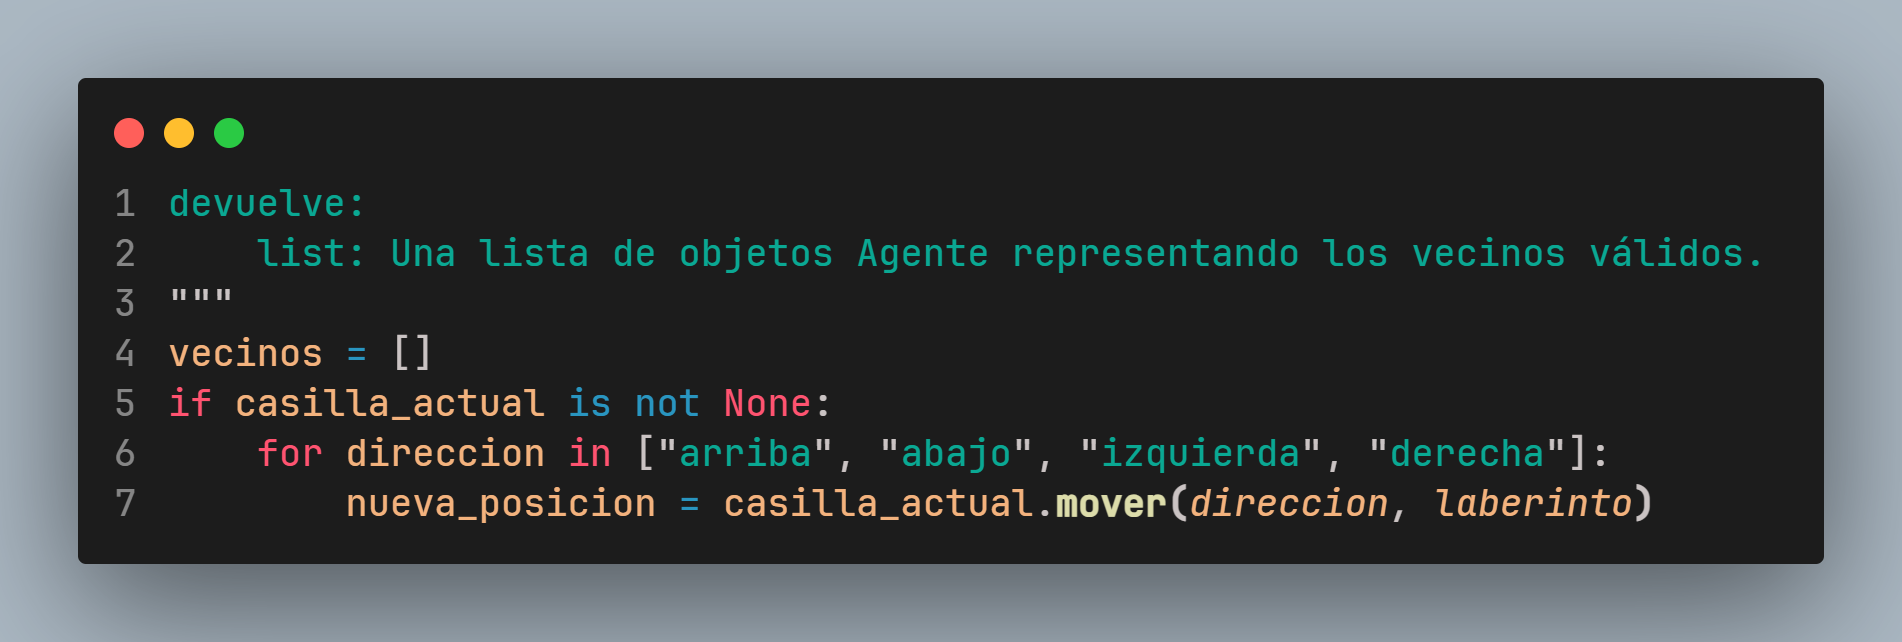
\includegraphics[width=0.65\linewidth]{IMA/Situacion1.png} 
    \caption{Codigo para cambiar la prioridad del agente en la busqueda de caminos.} 
    \label{fig:ejemplo} 
\end{figure}

Por ultimo, consideremos un laberinto de 7x7 con la característica de que la salida del laberinto no 
se encuentra accesible debido a que se encuentra rodeada de muros, es decir, no existe un camino para llegar a la salida.

\begin{figure}[H]
    \centering
    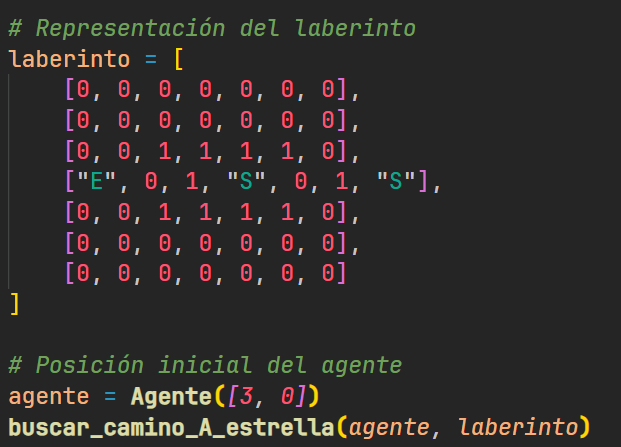
\includegraphics[width=0.5\linewidth]{IMA/Laberinto3.png} 
    \caption{Ejemplar para el agente, con salida inaccesible.} 
    \label{fig:ejemplo} 
\end{figure}

En este caso, el agente no encontrara un camino para llegar a la salida, por lo que el agente no encontrara una solución.

\begin{figure}[H]
    \centering
    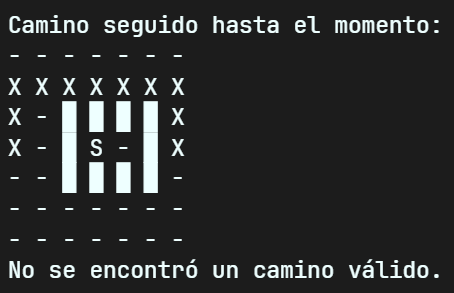
\includegraphics[width=0.5\linewidth]{IMA/RLaberinto3.png} 
    \caption{Momento en el que el agente no encuentra una solución.} 
    \label{fig:ejemplo} 
\end{figure}

Con fines academicos (esta visualizacion no refleja la implementacion, solo es ilustativo de la pagina \url{https://qiao.github.io/PathFinding.js/visual/} ), la siguiente imagen muestra el comportamiento del agente con el algoritmo A* en el laberinto, desde el inicio de la ejecución, 
el agente descarta a los vecinos de arriba y abajo por ser casillas más lejanas a la salida y se dirige a la derecha ya que es casilla que se encuentra más cerca de la salida.
Posteriormente sigue buscando casillas vecinas más a la derecha, hasta que encuentra muros, por lo que el agente opta por ir rodeando el muro hasta encontrar la salida.
Cuando finalmente encuentra una posible entrada al muro que rodea la salida, se da cuenta que no es posible llegar a la salida, por lo que el agente termina la ejecución.

\begin{figure}[H]
    \centering
    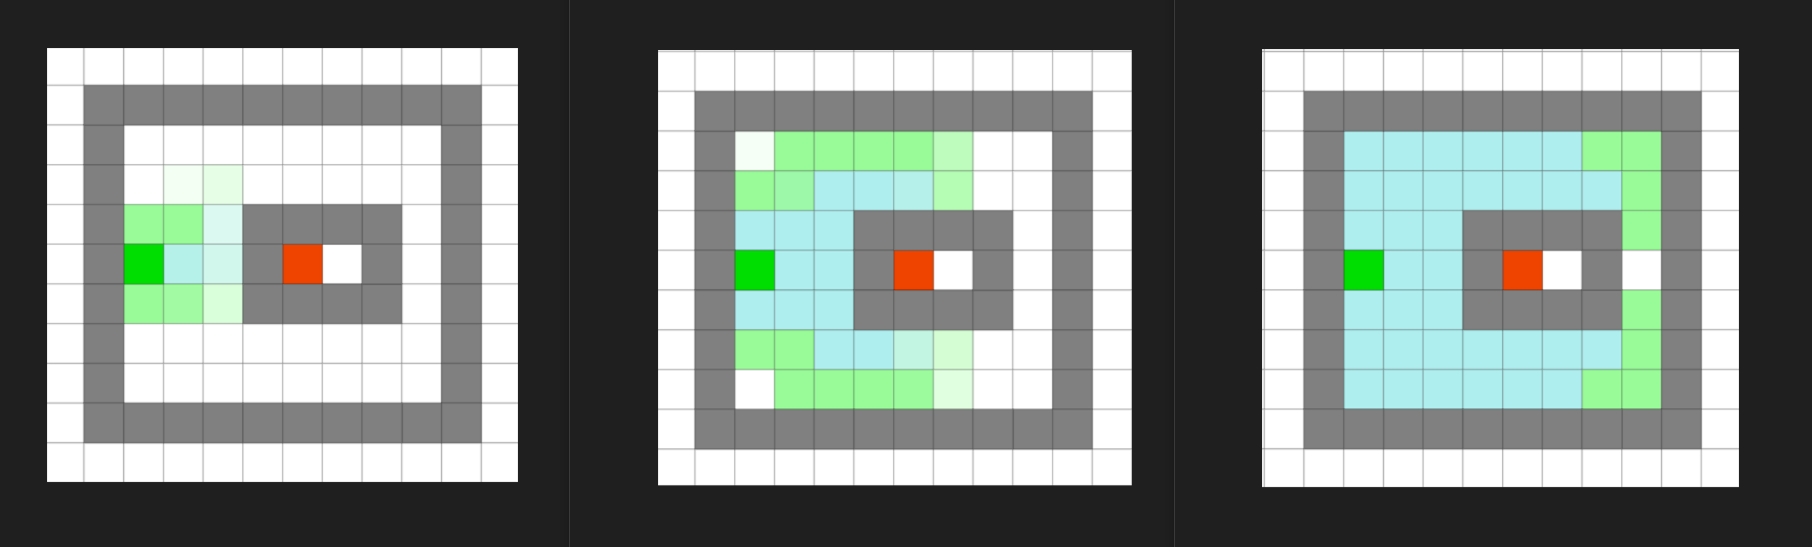
\includegraphics[width=0.9\linewidth]{IMA/RLaberinto3VCompleto.png} 
    \caption{Ejemplo ilustrativo de Algoritmo A* en el laberinto, con salida inaccesible.} 
    \label{fig:ejemplo} 
\end{figure}

\subsection*{Versiones del codigo}

En seguida haremos notar los cambios que se hicieron entre dos versiones de implementacion y el por que de estos cambios.

\begin{lstlisting}[language=Python, caption=Version 1: reconstruir_camino]
    def reconstruir_camino(casilla_actual):
    """
    Esta función reconstruye el camino desde la casilla actual hasta la posición inicial del agente.

    recibe:
        casilla_actual (Agente): La casilla actual.

    devuelve:
        list: Una lista que representa el camino desde la casilla actual hasta la posición inicial del agente.
    """
    camino = []
    while casilla_actual:
        camino.append(casilla_actual.posicion)
        casilla_actual = casilla_actual.padre

    return list(reversed(camino))
\end{lstlisting}

\begin{lstlisting}[language=Python, caption=Version 2: reconstruir_camino]
    def reconstruir_camino(casilla_actual):
    """
    Esta función reconstruye el camino desde la casilla actual hasta la posición inicial del agente.

    recibe:
        casilla_actual (Agente): La casilla actual.

    devuelve:
        list: Una lista que representa el camino desde la casilla actual hasta la posición inicial del agente.
    """
    camino = []
    while casilla_actual:
        camino.append(casilla_actual.posicion)
        casilla_actual = casilla_actual.padre

    camino = list(reversed(camino))
    print("Ruta seguida:")
    for posicion in camino:
        print(f"[{posicion[0]}, {posicion[1]}]")
    print("Se encontró la salida :D")  

    print("\nCamino encontrado:")
    for i in range(len(laberinto)):
        fila = ""
        for j in range(len(laberinto[0])):
            if [i, j] in camino:
                fila += "X "
            else:
                fila += "- "
        print(fila)

    return camino
\end{lstlisting}

{\tt Notemos que en la version 2 el cambio es mas que nada la salida por pantalla, es decir la ruta que el agente tomo para encontrar la salida, y ademas mosyramos el camino seguido por el agente, aquí iteramos sobre el laberinto y determinamos la posición del agente, si se encuentra dicha posición colocamos una \textbf(X), en caso contrario solo coloacamos una guion \textbf(-). Este cambio lo consideramos importante ya que como bien se dijo anteriormente hace que se mas visible, clara y permite que se pueda entender mejor como se llego a la salida.}

\begin{lstlisting}[language=Python, caption=Version 1: distancia_manhattan]
    def distancia_manhattan(nodo_actual, nodo_objetivo):
    """
    Calcula la distancia de Manhattan entre dos nodos.

    recibe:
        nodo_actual (Agente): El nodo actual.
        nodo_objetivo (Agente): El nodo objetivo.

    devuelve:
        int: La distancia de Manhattan entre los dos nodos.
    """
    diferencia_x = nodo_actual.posicion[0] - nodo_objetivo.posicion[0]
    diferencia_y = nodo_actual.posicion[1] - nodo_objetivo.posicion[1]
    distancia = abs(diferencia_x) + abs(diferencia_y)
    return distancia
\end{lstlisting}

\begin{lstlisting}[language=Python, caption=Version 2: distancia_manhattan]
    def distancia_manhattan(laberinto):
    """
    Calcula la distancia de Manhattan entre dos nodos.

    recibe:
        laberinto (list): El laberinto representado como una matriz

    devuelve:
        int: La distancia de Manhattan entre los dos nodos.
    """
    nodo_actual = punto_de_partida(laberinto) #Buscamos la posicion inicial del agente
    nodo_objetivo = salida_laberinto(laberinto) #Buscamos la salida del laberinto

    x, y = nodo_actual 
    w, z = nodo_objetivo
    
    distancia = abs(x - w) + abs(y - z) #Calculamos la distancia Manhattan dados dos puntos
    return distancia
\end{lstlisting}

Este cambio tambien es importante ya que notemos primero en la version 1 dependemos mucho de la posicion actual del agente(\textbf{nodo_actual}) y la posición de la salida(\textbf{nodo_obejtivo}) como parametros en cambio en la version 2, al eliminar esto hacemos uso de dos funciones \textbf{punto_de_partida} con esta obtenemos las coordenadas de la posición inical del agente y \textbf{salida_laberinto} con esta obtenemos las coordenadas de la salida del laberinto (si la hay), y notemos que al hacer este cambio hacemos que la funcion de distancia Manhattan sea mas versatil, es decir, podemos usarla en diferentes laberintos, pasando como parametro algún laberinto, y asi no modificar la funcion, con esto tambien añadimos que mejora la modularidad del codigo, haciendo que el codigo pueda ser usado en un futuro, y sea mas facil de comprender.

Las siguiente funciones son metodos auxiliares que nos ayudan a encontrar la posición inicial del agente y la salida del laberitno respectivamente.
Se realizo este añadido con la finalidad de que sea más fácil de entender y comprender como estamos buscando las coordenadas de la entrada y salida del laberinto, además de hacer que nuestro código sea mas flexible

\begin{lstlisting}[language=Python, caption=Función auxiliar: punto_de_partida]
    def punto_de_partida(laberinto):
    """
    Encuentra la posición inical del agente en el laberinto

    Recibe:
        laberinto (list): El laberinto representado como una matriz.

    Devuelve:
        tupla: La posición(coordenadas) inicial del agente
    """
    try:
        for i in range(len(laberinto)):
            for j in range(len(laberinto[0])):
                if laberinto[i][j] == "E":  # Comprobamos si encontramos la entrada
                    return (i, j)  # Devolvemos las coordenadas 
    except ValueError:
        print("No se encontró la salida del laberinto.")
\end{lstlisting}

\begin{lstlisting}[language=Python, caption=Función auxiliar: salida_laberinto]
    def salida_laberinto(laberinto):
    """
    Encuentra la posición de la salida del laberinto

    Recibe:
        laberinto (list): El laberinto representado como una matriz.

    Devuelve:
        tupla: La posición(coordenadas) de la salida del laberinto.
    """
    try:
        for i in range(len(laberinto)):
            for j in range(len(laberinto[0])):
                if laberinto[i][j] == "S":  # Comprobamos si encontramos la salida
                    return (i, j)  # Devolvemos las coordenadas 
    except ValueError:
        print("No se encontró la salida del laberinto.")
\end{lstlisting}

Otros pequeños cambios que se hicieron fue que en lugar se usar una condición para ejecutar el algoritmo, eso se hizo simpelemnete por comodidad y que sea mas claro.

\begin{lstlisting}[language=Python, caption=Versión 1: ejecución algoritmo]
	if camino:
    	print("Camino encontrado:", camino)
	else:
    	print("No se encontró un camino válido.")
\end{lstlisting}

\begin{lstlisting}[language=Python, caption=Versión 2: ejecución algoritmo]
	agente = Agente([0, 0])
	buscar_camino_A_estrella(agente, laberinto)
\end{lstlisting}

